\chapter{Definice problému}
Hlavním problémem při zpracování dat z kapslové endoskopie je jejich nepřeberné množství. Lékaři musí projít obrázek po obrázku, což pro ně znamená velkou časovou náročnost. Ta by šla využít při řešení konkrétního problému jinak než jeho hledáním. Je proto potřeba nalézt takové řešení, které by tuto práci maximálně zjednodušilo a usnadnilo.

Vyvinutá aplikace by měla být schopná vyhodnotit záznam a detekovat možné krvácení ve střevech. Data z kamery jsou extrahována do proprietárního formátu každého výrobce, ze kterého pak lze extrahovat sekvenci nafocených obrázku buď do formátu \gls{glos:AVI}, ale s velkou kompresí, a tudíž ztrátou informací, anebo do sekvence po sobě jdoucích \gls{glos:JPG} obrázku beze ztráty kvality. Aplikace přijme tato data jako vstup. A na výstupu pak bude informace, zda se v daných datech nachází krvácení. 

\begin{figure}[h]
	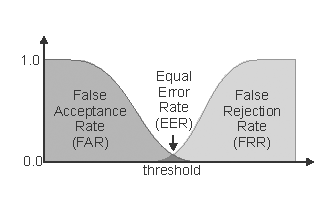
\includegraphics[scale=0.8]{eergraf}
	\centering
	\caption{EER graf \cite{gumption:}\label{fig:eergraf}}
\end{figure}

Je nutné popsat nebo definovat hledaný objekt tak, aby se za pomocí zpracování obrazu dal objekt nalézt s co největší přesností a nejmenším počtem chyb. Bylo by tedy potřeba nalézt \gls{glos:EER} mezi \gls{glos:FAR} a \gls{glos:FRR} viz obrázek, \ref{fig:eergraf}. Jelikož je v biomedicíně nutné nalézt všechny pozitivní objekty a ideální stav je 0\% \gls{glos:FRR}, tak se dá akceptovat větší míra \gls{glos:FAR}. Jinými slovy - je lépe označit více objektů, i když některý z nich může být chybou, než-li minout snímek, v němž se vyskytuje problém.

\begin{figure}[h]
	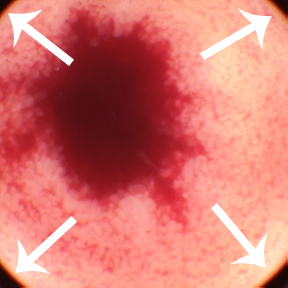
\includegraphics[scale=0.6]{anomalie}
	\centering
	\caption{Anomálie při sběru dat \label{fig:anomalie}}
\end{figure} 

Největším problémem je definování hledaného objektu, neboť kvalita dat není kvůli nízkému rozlišení kamer příliš velká. A navíc, každý výrobce má specifické barevné schéma, rozlišení a artefakty, které vznikají při sběru dat. Ukázkou může být obrázek \ref{fig:anomalie}, jenž znázorňuje, že tato kamera má u okrajů viditelný pruh barev, který pak může způsobovat problémy. V datech se také vyskytuje spousta anomálií, jež komplikují rozpoznávání objektu (různé odlesky, zbytky potravy, podobné barevné rozpoložení, …). Bude tedy potřeba zkombinovat více metod pro dosažení co nejlepšího výsledku.


V následujících kapitolách jsou uvedeny související vědecké práce, které se zabývají definováním stejného problému.

\section{Detection of bleeding in wireless capsule endoscopy using range ratio color \cite{detection}}
V článku „Detection of bleeding in wireless capsule endoscopy images using range ratio color“ výsledky byly klasifikovány na možnosti krvácení či neoznačení výskytu krve. Byla zde použita platforma C\#.

Analýza obrazu probíhala vždy ve dvou krocích. První krok efektivně rozdělí vstupní videa na ty, které obsahují výskyt krvácení a naopak. V druhém kroku následuje samotná detekce krvavých míst a klasifikace aktivních vzorků krvácení. První testovanou funkcí byla barva, která přinesla pouze selhání. Použitý algoritmus nepřinesl výsledky, které se očekávaly. Druhou testovací funkcí bylo použití parametrů poměr – barva. Tato funkce přinesla lepší výsledky než první. Oba dva algoritmy probíhaly téměř stejně - testovaly se všechny pixely na obrázku o proti podmínce, která se lišila v závislosti na použitém algoritmu. Podmínky je možné vidět na obrázku \ref{fig:clanekalg}.
\begin{figure}[h]
	
\includegraphics[scale=0.7]{clanekalg}
	\centering
	\caption{Použité algoritmy.\cite{detection} \label{fig:clanekalg}}
\end{figure} 

Bylo testováno 100 \gls{glos:WCE} snímků pořízených na různých částech trávícího traktu. Při použití stanovených podmínek byl výsledek první funkce s přesností stanoven na pouhých 48\%. Avšak druhá funkce umožnila povýšit přesnost až na 98\%. Přehled dosažených výsledků u obou metod můžeme shledat v tabulce \ref{tab:detection}.

\begin{table}[h]
	\centering
	\begin{tabular}{|l|c|c|c|c|}
		\hline
		\bf Klasifikace & \multicolumn{1}{l|}{\begin{tabular}[c]{@{}l@{}}\bf Detekovaných \\ \bf snímků s krví\end{tabular}} & \multicolumn{1}{l|}{\begin{tabular}[c]{@{}l@{}}\bf Detekovaných\\ \bf snímku bez krve\end{tabular}} & \multicolumn{1}{l|}{\begin{tabular}[c]{@{}l@{}}\bf Celková\\ \bf správná hodnota\end{tabular}} & \multicolumn{1}{l|}{\bf Přesnost} \\ \hline
		Pouze červená barva & 2 & 98 & 48 & 45\% \\ \hline
		Rozsah barev & 52 & 48 & 98 & 98\% \\ \hline
	\end{tabular}
	\caption{Výsledku algoritmů. Přeloženo z \cite{detection}}
	\label{tab:detection}
\end{table}
\FloatBarrier

Závěrem můžeme konstatovat, že tato metoda je jednoduchá a přesná.

\section{„A technique for blood detection in wireless capsule endoscopy images \cite{technique}}
Článek „A technique for blood detection in wireless capsule endoscopy images“ se zabývá způsobem rozlišování mezi běžnou sliznicí a regionů krvácejících tkání. Opět pomocí WCE snímků. Tohoto způsobu bylo dosaženo identifikaci lišících se oblastí. Lišit se mohou prostorové nebo spektrální charakteristiky od svého okolí. Oblasti pokryté krví jsou považovány za izolované cíle na pozadí. Celý tento proces je označen za detekce anomálií. 

Detekce anomálií se provádí prostřednictvím testování hypotéz daného problému. V případě detekce krve se používá pixel (anomální pixely) při reprezentaci barvy a stanovené hodnoty kovarianční matice. Vše se provádí za předpokladu stacionárního procesu v pozadí. Tento předpoklad se potlačuje především při výskytu vzduchových bublin či organických zbytků. Z tohoto důvodu je aplikován předzpracující stupeň – tedy příprava dat pro detekci anomálií a následně po dokončení spuštění RX algoritmu. Postup vícestupňové detekce krve je následující:

\begin{enumerate}
	\item Odstranění tmavých míst a detekce červených pixelů -
	V první fázi se vyloučí regiony, které nejsou detekovány jako užitečné (střevní šťávy, tmavé oblasti) a vyberou se pouze regiony s výskytem krve. Druhá fáze je rozdělena na další pod části. Nejprve se odstraní pixely tmavé velmi barvy, poté jsou červené pixely detekovány jako potencionální krev. Střevní obrazy dokáží poukázat na vysoce červený odstín. Výjimkou jsou snímky pořízené z oblasti tlustého střeva, kde jsou dominantní barvy oranžové až žlutozelené vzhledem k výskytu fekálních ostatků. 
	\item Hrana maskování -
	 Abychom snížili výskyt anomálií, aplikujeme okrajové maskování. Hrany jsou získány za pomocí Mumford-Stashova algoritmu jako výsledky funkční minimalizace problému. Obraz je dále předán dalšímu zpracování.
	\item Detekce krve -
	V tomto okamžiku jsou shromážděny výsledky z již předchozích fází. Kombinací těchto dvou způsobů třídění dat dosáhneme lepší spolehlivosti konečného výsledku. Kombinací detekcí červených barev, detekcí anomálií a maskováním získáme nekrvácející oblasti. 
	\item Morfologické operace -
	Krvácející oblasti se nejeví jako malé a izolované oblasti. Na základě tohoto faktu je užitečné odebrat izolované anomálie pixelů. Na obrázku \ref{fig:clanepostup} můžeme shledat konečnou podobu detekce krve.
\end{enumerate}

\begin{figure}[h]
	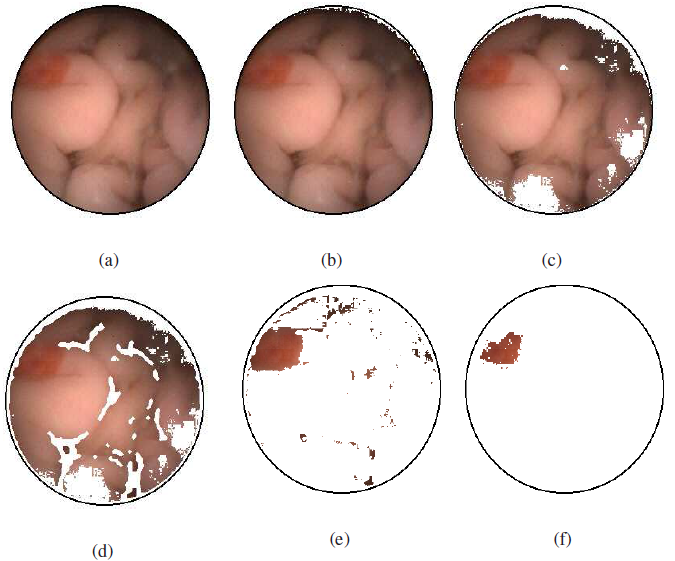
\includegraphics[scale=0.5]{clanekpostup}
	\centering
	\caption{Postup algoritmu a.originální obraz;b.odstranění černých pixelů;c.detekce červené barvy;d.maskování hran;e.detekce krve;f.výsledek RX algoritmu \cite{technique} \label{fig:clanepostup}}
\end{figure} 
\FloatBarrier
	
Simulace byly prováděny na 11 sekvencích (8 patologických případů, 3 zdraví jedinci). Každá sekvence se skládá ze 101 rámců o velikosti 256 x 256 pixelů. Přesnost výsledků byla hodnocena za pomocí standardních kriterií v biomedicíně (upřesněno v kapitole \ref{sec:metodologie}). Na obrázku \ref{fig:clanektabulka} můžeme shledat výkonnost navrhovaného algoritmu.

Výsledky ukázaly vyšší citlivost a specifičnost experimentálních navrhovaných způsobů. Tím pádem se dosahuje uspokojivých výsledků. Nesmí se však opomenout fakt, že použité sekvence jsou komprimovány. V důsledku komprimace dochází k negativnímu ovlivnění zaváděné komprese. Budoucí vývoj bude aplikovat konkrétní algoritmus na ověření nekomprimovaných dat a vykořisťování korelace mezi sousedními rámy a to vše za účelem zlepšení výkonu detekce.

\begin{figure}[h]
	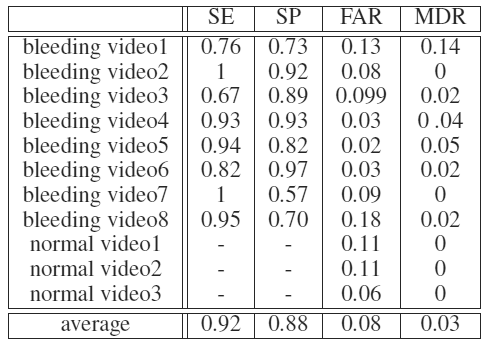
\includegraphics[scale=1]{clanektabulka}
	\centering
	\caption{Výsledky RX algoritmu \cite{technique} \label{fig:clanektabulka}}
\end{figure} 
\FloatBarrier

\section{Problémy detekce artefaktů v reálném prostředí}
Z vědeckých článků je zřejmé, že na vybrané databázi testovaných vzorků dosáhli celkem dobré úspěšnosti. Nicméně, nabízená řešení jsou příliš orientována na detekci dle barvy. V prvním případě se bude v reálných datech vyskytovat mnoho \gls{glos:FP}, protože na každém snímku se objeví alespoň jeden pixel, který bude zapadat do daného rozsahu.

V druhém článku je přidáno odstranění nechtěných anomálií po detekci barev. To může mít za následek zpřesnění výsledků, neexistuje zde však další mechanismus nezávisle na barvě, např. detekování samotného tvaru.

Z článku lze vycházet, jelikož přece jen detekce barvy je stěžejní pro určení krve. Pro přesnější výsledek je však nutné hledaný objekt definovat za pomocí detekce tvaru. Detekováním tvaru bude možné popsat rozdílnost od pozadí (lidský mozek zpracovává informace podobně, je schopný detekovat tvar objektu, aniž by záleželo na barvě).